%% ----------------------------------------------------------------------------
% BIWI SA/MA thesis template
%
% Created 09/29/2006 by Andreas Ess
% Extended 13/02/2009 by Jan Lesniak - jlesniak@vision.ee.ethz.ch
%% ----------------------------------------------------------------------------
\newpage
\chapter{Semi-supervised image segmentation using RFs in a Bayesian framework }
The philosophy behind semi-supervised learning is to propagate the label information from labeled to unlabeled data. Image segmentation can be seen as a classification problem which consists of assigning a class label to each pixel. For our task of binary segmentation, this means classifying each pixel as foreground or background. For our task of image segmentation, we make use of the partial annotations as \textit{scribbles}. Scribbles are pixels in the image annotated by experts as foreground or background. In this chapter, we use the Random forests for our segmentation task. We train the Random forests using scribbles and try to achieve similar accuracy as we obtained with CNNs in previous chapter. One major contribution of this chapter is analysis of effect of scribbles on accuracy. We designed few experiments to train RF with varying quality and quantity of scribbles, and observed the effect of these variations on segmentation accuracy. In addition, we improve the accuracy of RF by use of variational methods.

\section{Random Forest}
We can find a lot of research using RF for the binary image segmentation. Eugster \cite{dominic} explains the use of RF for the segmentation of microscopic images. This chapter is an extension of methods used by Eugster. For training RF, we compute set of features in Python. We compute different features ranging from simple Sobel edge detectors to higher level Gabor filters. The choice of features was made according to WEKA \cite{weka} toolset of FIJI \cite{fiji} plugin. These are set of 2D features and perform well for microscopic images. We compute different type of features for a range of sigmas, which gives 69 feature maps for a single image. The use of all 69 feature maps increases computational cost significantly, and also increases the training and testing time of RF. In the thesis by Eugster \cite{dominic}, we can find details of feature selection to choose N best features and use these N featrues to obtain an optimal balance between computational cost and accuracy. Similar to Eugster, we choose N best features and significant number of trees such that increasing the features or trees does not change the results significantly. This can be seen in figure 3.1. We can observe that for a given annotation budget i.e. fixed amount of scribbles, the segmentation measure does not change significantly for more than 30 trees and for more than 20 features. Therefore, for all experiments using RF, we use 20 best features and 30 trees for training. In following sections, we focus on how to get best results for given annotation budget and thus, use the fixed number of features and trees to generate segmentation masks. 

\begin{figure}[h!] \label{fig:rf_complex}
\begin{tabular}{cc}
 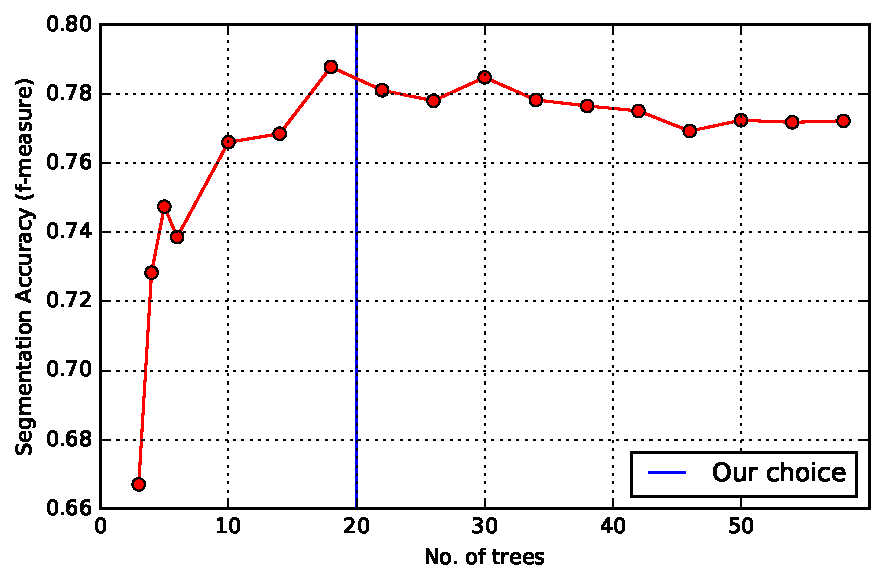
\includegraphics[width=0.5\linewidth]{figures/diff_features.pdf} & 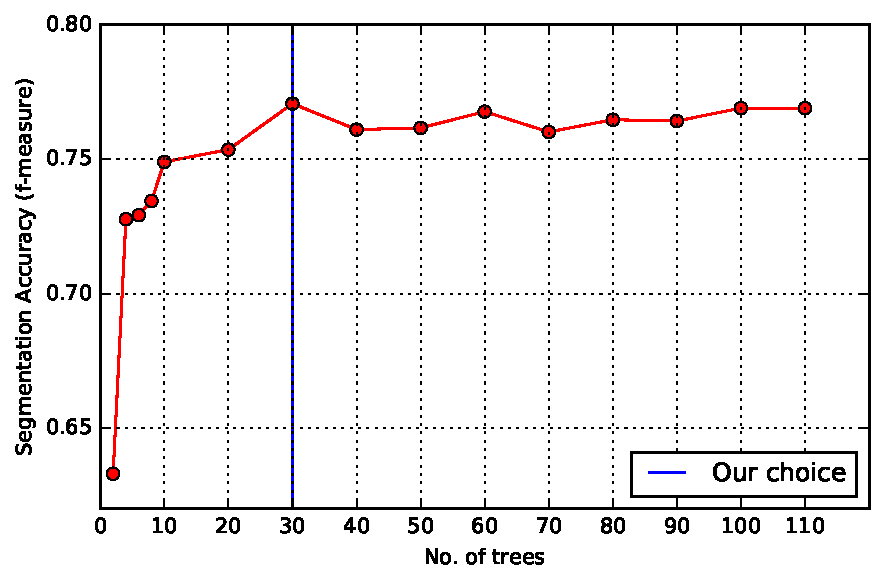
\includegraphics[width=0.5\linewidth]{figures/diff_trees.pdf} \\
  (a)  & (b) \\
\end{tabular}
\caption{Plot of segmentation measure vs changing complexity of RF: (a) with features, (b) with trees}
\end{figure}

\section{Best use of annotaion budget}
Earlier research for segmenting images in classical computer vision problems has mostly been focused on improving the segmentation accuracy or improving the performance speed. This can be understood as the annotating the ground truth is not as difficult and time consuming as it is in microscopic images. For our scenario, the use of annotation budget to produce best results is of utter most importance. Due to these reasons, we try to observe the effect of annotaion budget on segmentaion accuracy. We try to observe this by varying quality and quantity of scibbles. The quality of scribbles is related to the position of scribbles or where to scribble i.e. the scribble can be near to boundary of object or in the inner body of the object. The quantity of scribbles correspond to amount of pixels annotated. Thus, we try to obtain optimal quality and quantity of scribble needed in order to obtain a significant level performance.

\subsection{Where and how much to scribble?}
In general, we believe that more the training data we provide, more we can improve the results. Does this hold for partial annotation such as scribbles? If we go on increasing the pixels annotated arbitrarily, will it improve the segmentation mask or we have to use our labeling effort intelligently to improve results?


\begin{figure}[h!] \label{fig:scribbles}
\begin{tabular}{cc}
 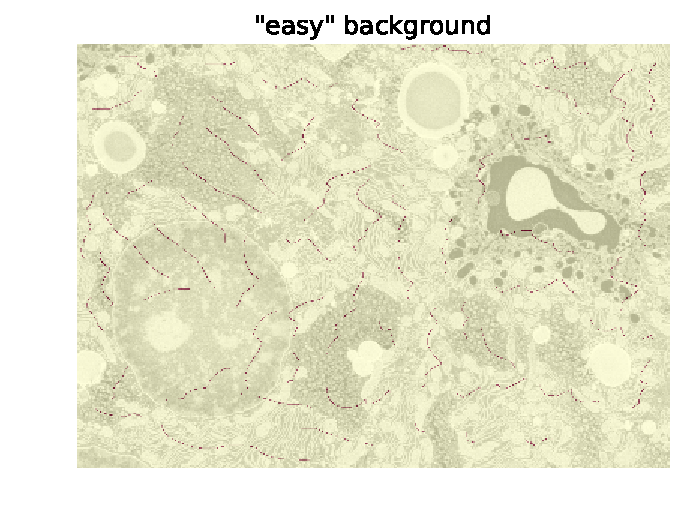
\includegraphics[width=0.5\linewidth]{figures/easy_bg.pdf} & 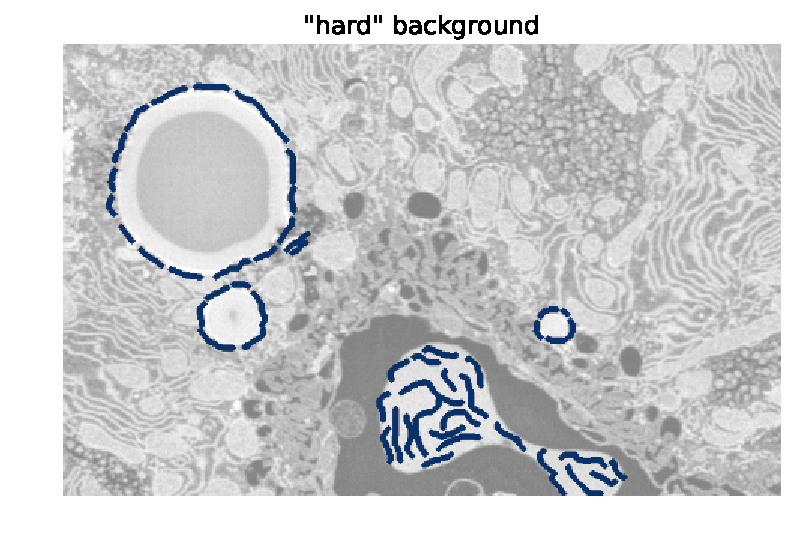
\includegraphics[width=0.5\linewidth]{figures/hard_bg.pdf} \\
 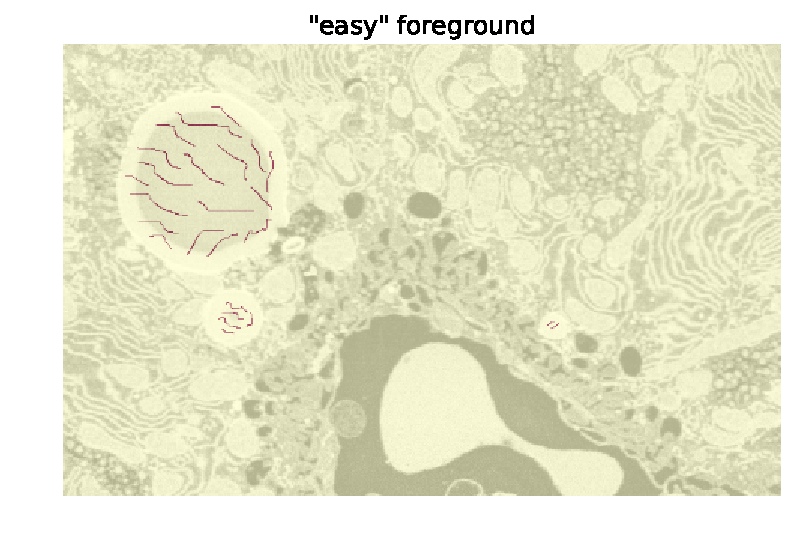
\includegraphics[width=0.5\linewidth]{figures/easy_fg.pdf} & 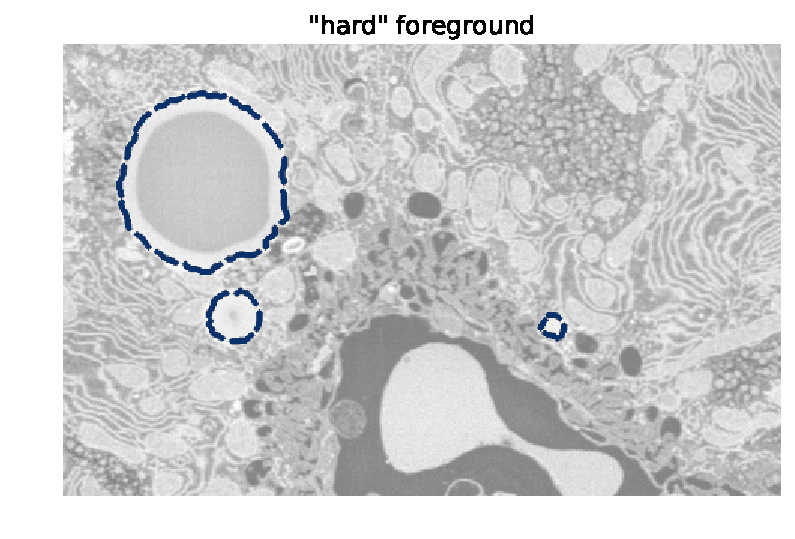
\includegraphics[width=0.5\linewidth]{figures/hard_fg.pdf} \\ 
\end{tabular}
\caption{Manual scribbles in "easy" and "hard" annotation classes}
\end{figure}

We designed an experiment by dividing our set of foreground and background scribbles into 2 annotation classes: easy and hard scribbles. We classified the scribbles as "easy" and "hard" depending on the effort required to annotate these pixels. For example, the pixels are difficult to annotate near the boundary of foreground and background, and we classify these pixels as "hard", as shown in figure 3.2. We manually scribbled image for both "easy" and "hard" annotation subclasses. Then, we trained and tested RF on one image by increasing percentage of scribbles belonging to "easy" foreground and background class. After we have used all scribbles belonging to "easy" annotation class, we added scribbles from "hard" annotaion class for both foreground and background. The increment was made in percentage w.r.t. the total amount of scribbles we have. At each step of increment, only new scribbles were chosen randomly on the top of already chosen pixels. Also, as we increased the amount of scribbles we tried to maintain a ratio between foreground and background pixels. The ratio was choosen proportional to ratio of total foreground and background pixels. To measure the segmented accuracy, we comapre the segmentation mask for the same slice, on which the pixels were annotated for training RF. For measuring segmentation accuracy, the output probability mask from RF was thresholded using a value of 0.5.

\begin{figure}[h!] \label{fig:easy_hard}
\centering
 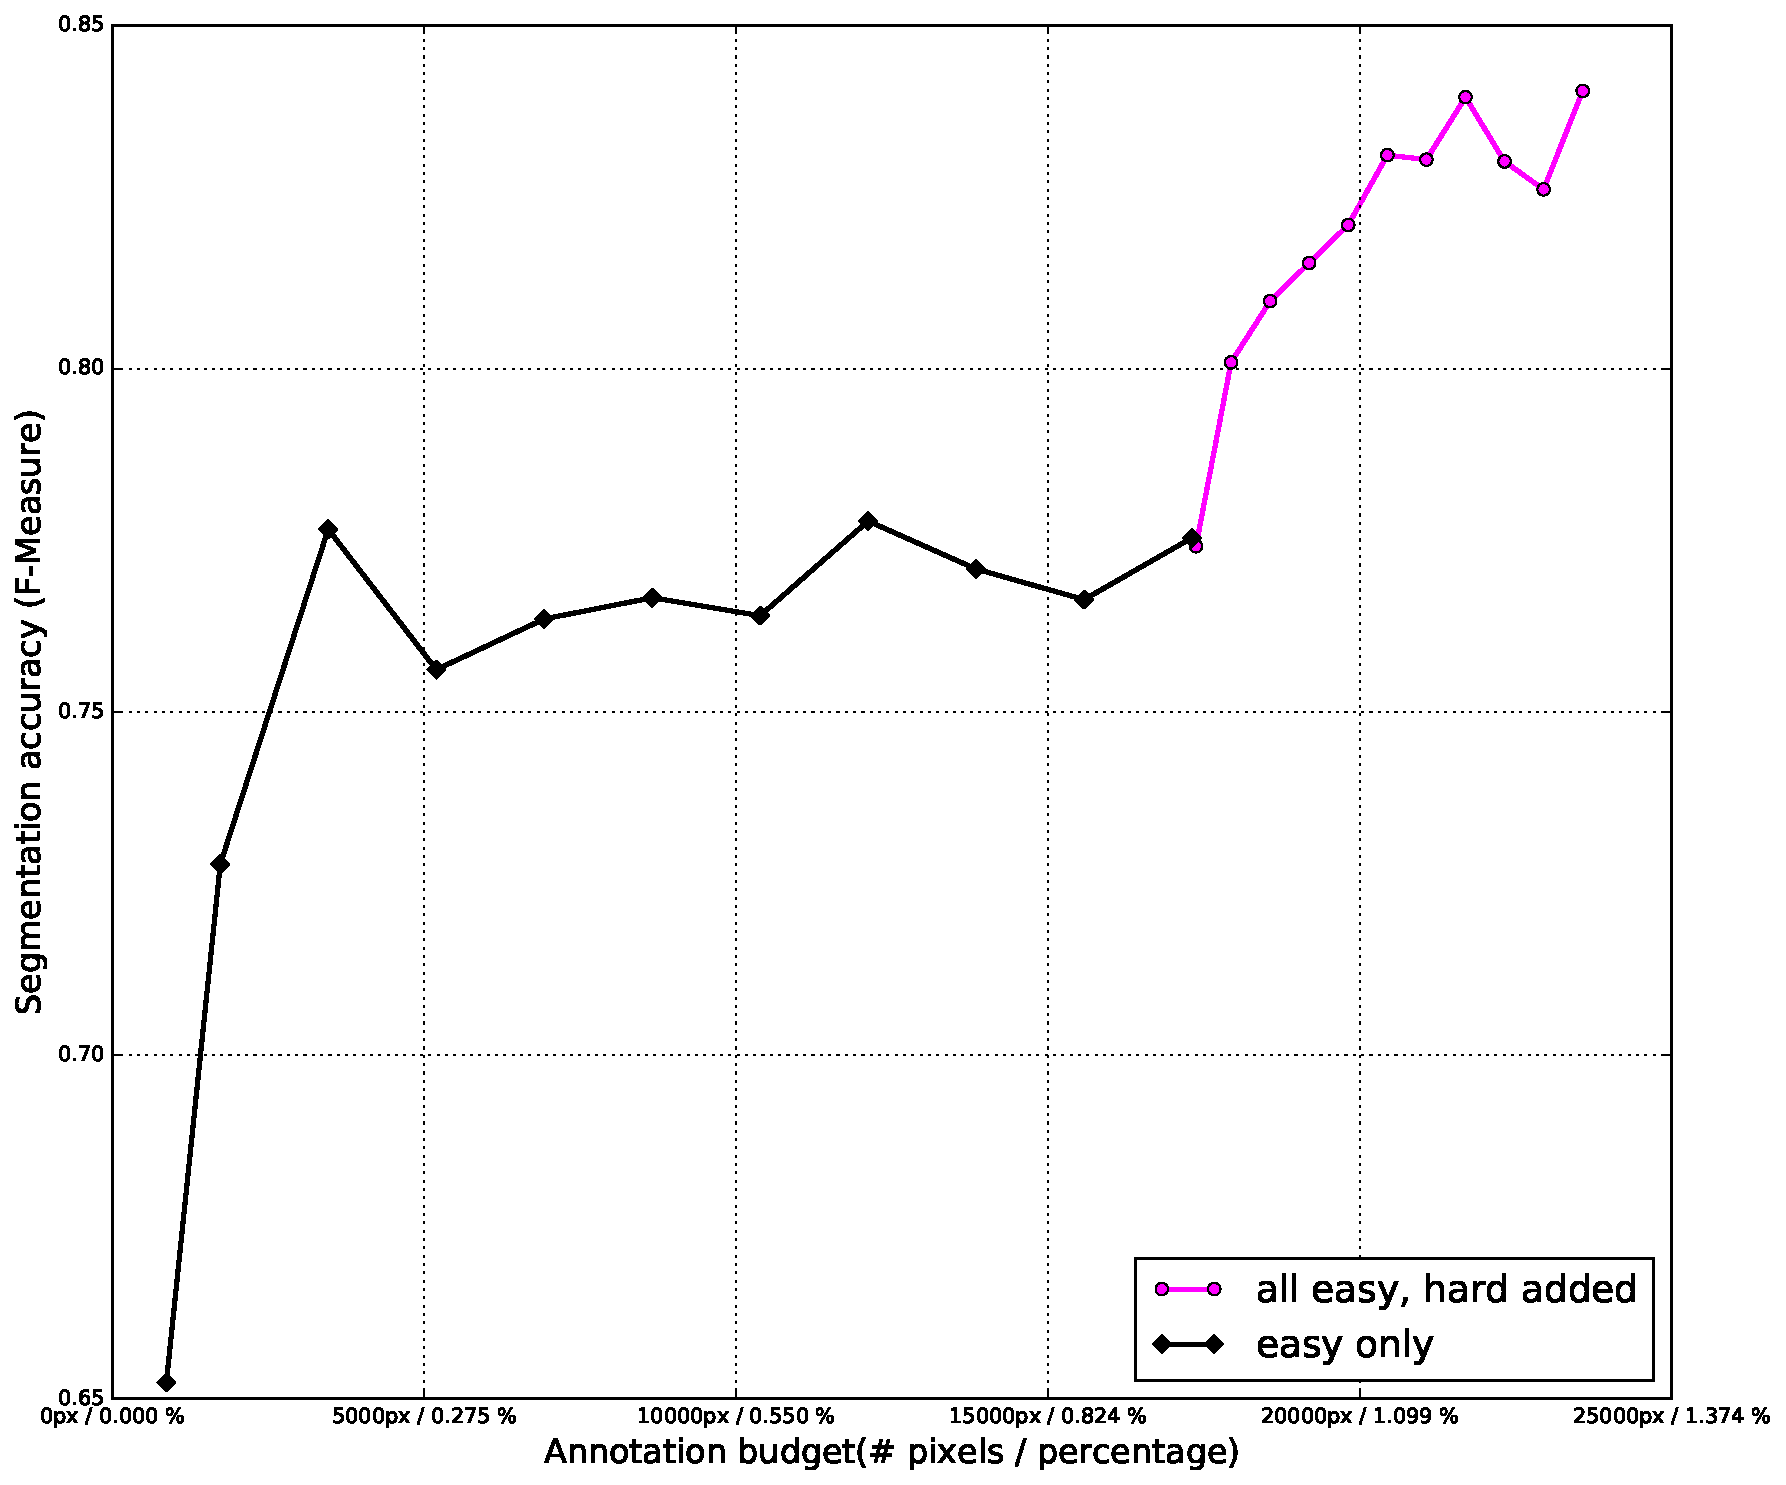
\includegraphics[width=0.73\linewidth]{figures/rf_easy_hard.pdf}
\caption{Plot of segmentation measure vs annotation budget. The black curve shows the increment of scribbles from the "easy" annotaion class. The pink curve shows the addition of scribbles from the "hard" annotaion class. The percentage in x-axix corresponds to amount of pixels w.r.t. to total pixels in image.}
\end{figure}

The result can be observed in figure 3.3. In the figure, we can observe that after a total of 3000 pixels (10\% of "easy" scribbles) selected from "easy" foreground and background, the segmentation accuracy does not change significantly. The segmentation accuracy varies between 0.73 to 0.76. This implies that further addition of "easy" scribbles do not provide any extra information to RF. A boost in accuracy can be observed, once we add "hard" scribbles after all available "easy" scribbles were used. We can observe that we are able to achieve accuracy of 0.84 by a small annotation budget of around 25000 pixels in an image of size This shows that the best results can be obtained by adding "hard" scribbles over a certain fixed percentage of "easy" scribbles. Looking at the plot and keeping the insignificant variation in accuracy after 3000 pixels, it feels best to add the pixels from "hard" scribbles after initial amount of 3000 "easy" scribbles. We except a similar boost in accuracy and makes best use of our annotaion budget. We tried this and results can be observed in figure 3.4.

\begin{figure}[h!] \label{fig:easy_hard1}
\centering
 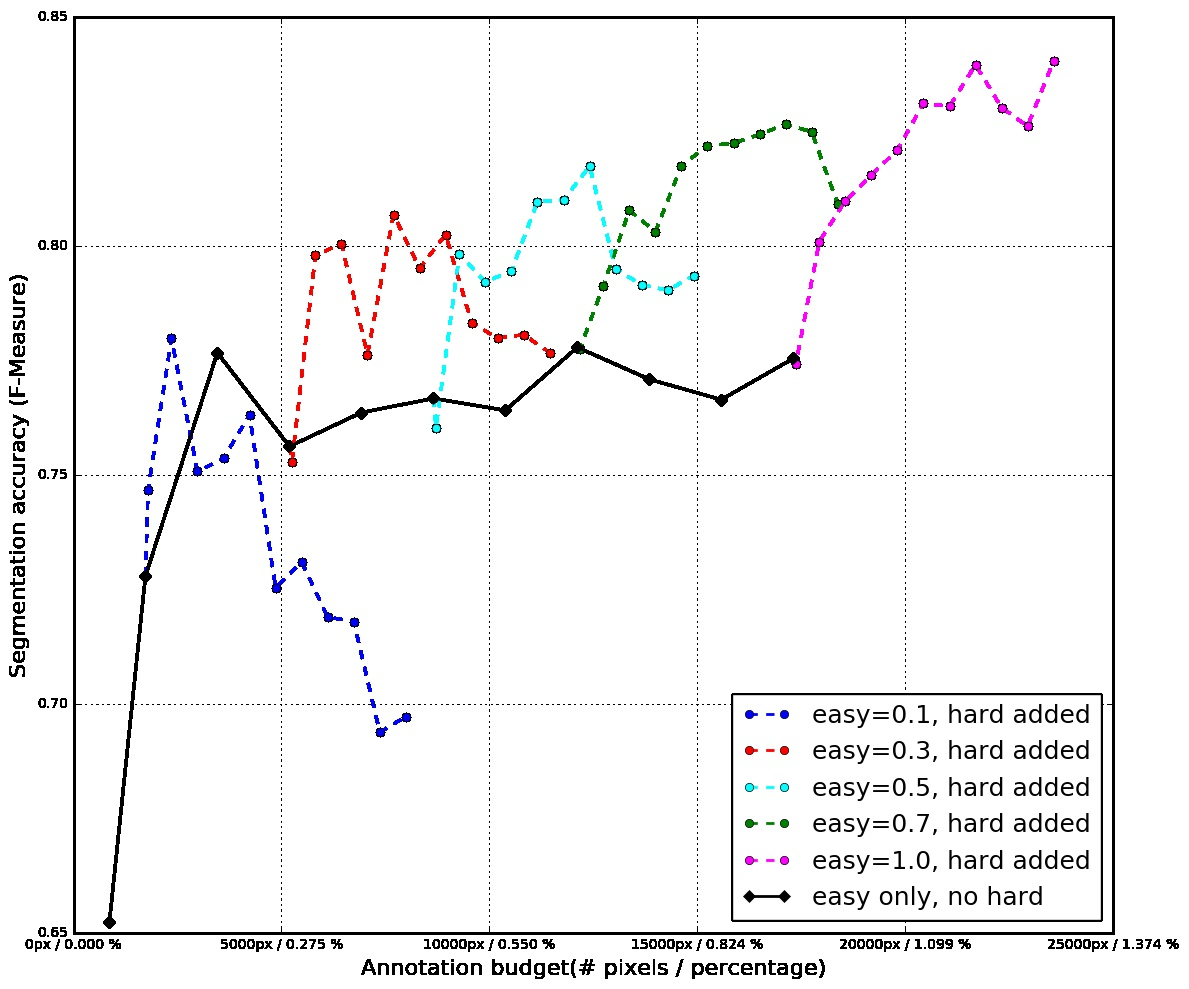
\includegraphics[width=0.85\linewidth]{figures/pres/rf_easy_hard.jpg}
\caption{Plot of segmentation measure vs annotation budget. Different curves show addition of scribbles from "hard" annotaion class, starting with different fixed amount of "easy" annotation class.}
\end{figure}

In figure 3.4, the addition of "hard" scribbles on top of 0.15\% (3000 pixels) of initial "easy" scribbles did not produce a boost as we expected. Instead of observing a continuous boost with addition of "hard" scribbles, we observed a fall in performance (dark blue plot in figure 3.4). This may be due to lack of enough "easy" scribbles and RF starts training its trees to focus more on "hard" scribbles. We repeated the addition of "hard" scribbles for different fixed amount of initial "easy" scribbles. We started seeing a significant improvement similar to earlier boost, when we utilized with 70\% of all "easy" scribbles to train RF (green plot in figure 3.4). We were able to achieve best f-measure score of 0.83 in comparison of 0.84 achieved with 100\% usage of "easy" scribbles (See green and pink plot in figure 3.4). The accuracy of 0.83 was achieved with use of only 1\% of total pixels in image. This was possible only because of quality of scribbles used. We can not achieve this accuracy if we annotate same amount of scribbles arbitatrily. Thus, the question arises how to decide the point of addition of "hard" scribbles and amount of "hard" scribbles to be added. The other observation is that continuous addition of "hard" scribbles do not always improve the results. We require an optimal balance between "easy" and "hard" scribbles. It is difficult to decide the position and quantity of scribbles prior to training RFs. 

\subsection{Iterative semi-interactive approach}
We observed the need of using our annotation budget intelligently to get the best performance out of it. But, we observed the problem of deciding on how many "easy" and "hard" scribbles are needed to achieve best results. For our problem, we divided the scribbles as "easy" and "hard" according to labeling effort, but this division for scribbles may not be same from point of view of the RFs. Apriori, we don't know which pixels will be difficult for the Random forest to classify correctly. The above mentioned two problems can be solved by annotating pixels iteratively to improve results. We can iterate the annotation at least once, to understand which pixels are difficult for RF to classify. We show the improvement in the result by doing one iteration in figure 3.5. We can observe that the scribbles are very few to produce a good result. Still, we can observe improvement in f-measure from 0.76 to 0.80 for increasing the annotation budget from 7500 pixels to 10900. Although the increment looks small, but we can observe the improvement at boundary in the large vesicle in left-top corner of the image. Thus, we can say that we can get a significant improvement with few iterations, even if we add small amount of pixels every time.
\begin{figure}[h!] \label{fig:semi-rf}
 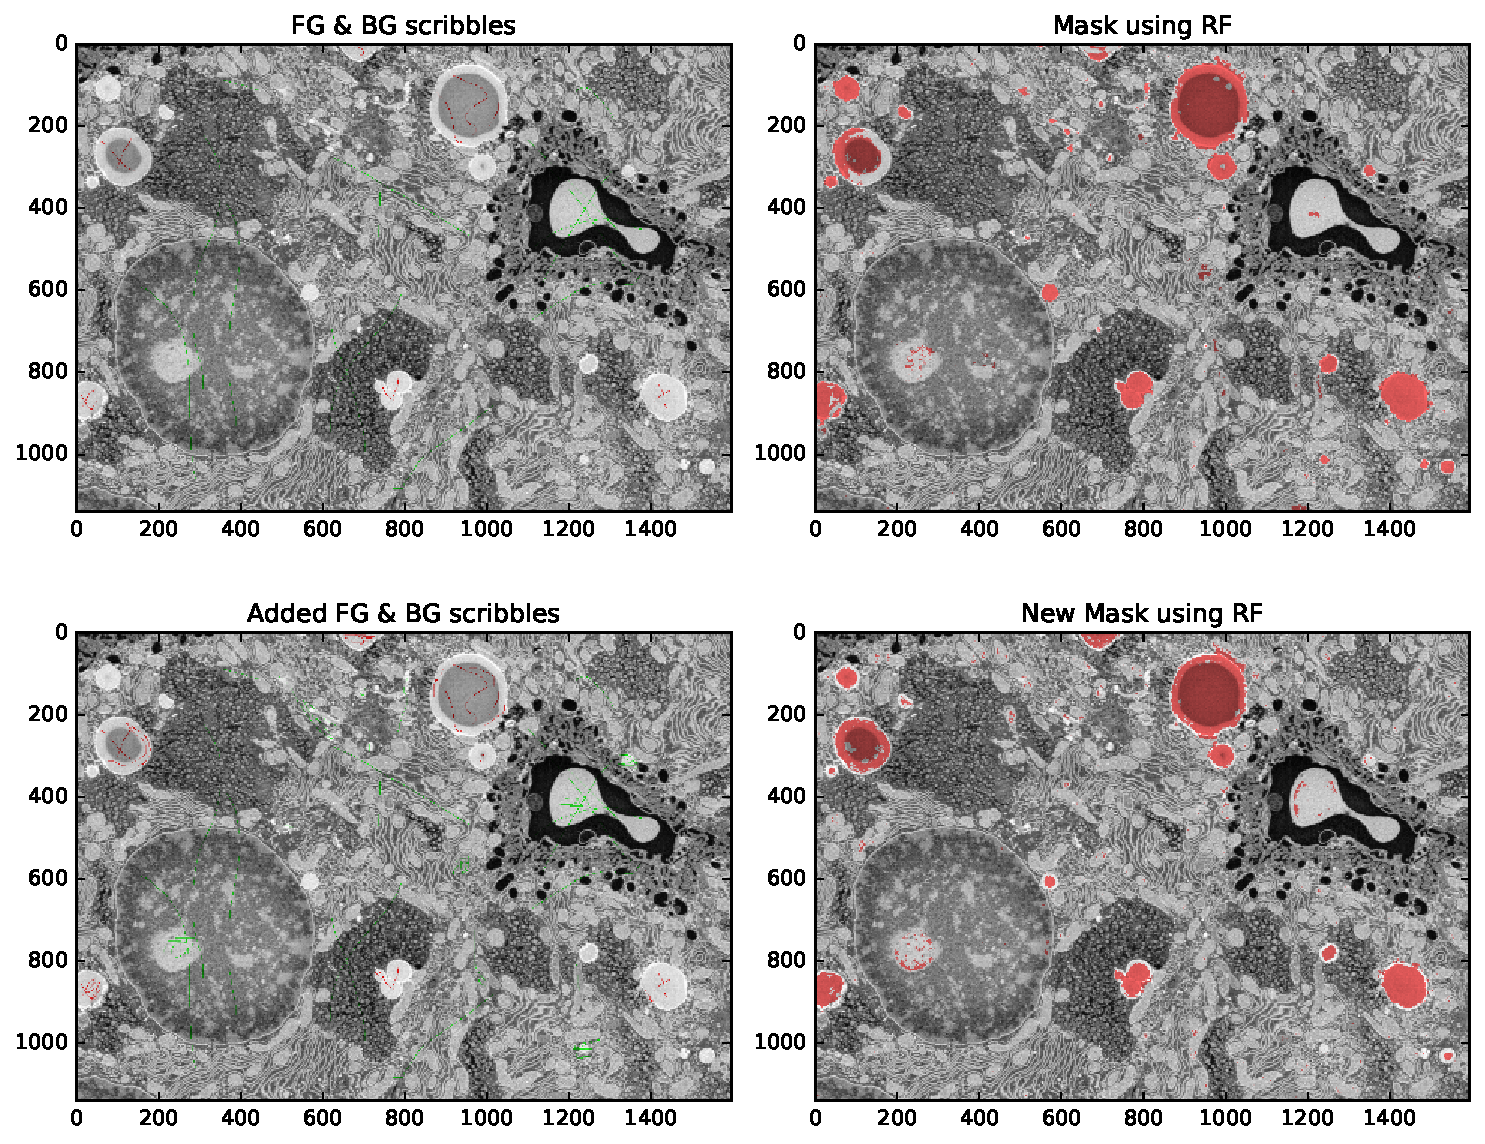
\includegraphics[width=1.0\linewidth]{figures/semi_inter_rf.pdf}
\caption{Semi-interactive segmentaion with one interaction. The bottom-left image shows scribbles added after first interaction using previously generated mask. Red: foregroud, Blue: background}
\end{figure}

The use of iterative semi-interactivity gives the best result for given annotation budget, but there is a limit on accuracy that can be achieved by using only RFs. The output mask of RF is noisy and uncertain. The uncertainty lies in the inability to classify maximum of pixels as foreground and background, as shown in figure 3.5(a). The histogram shows the distribution of probability of pixel to be foreground values for the complete image. It can be seen that a large number of pixels are not given a probability of 0 (background) or 1 (foreground). In figure 3.5(b), we can observe varying results for different threshold applied on probability mask obtained from RF. RF acts as a classifier and classifies each pixel but we need to group these pixels into objects for segmentation. 
\begin{figure}[h!] \label{fig:uncertain}
\begin{tabular}{cc}
 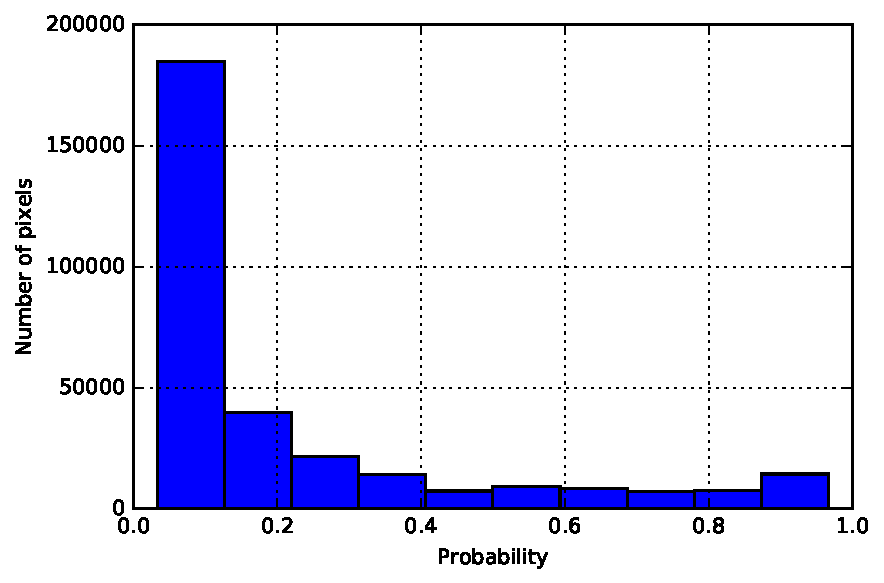
\includegraphics[width=0.5\linewidth]{figures/hist.pdf} & 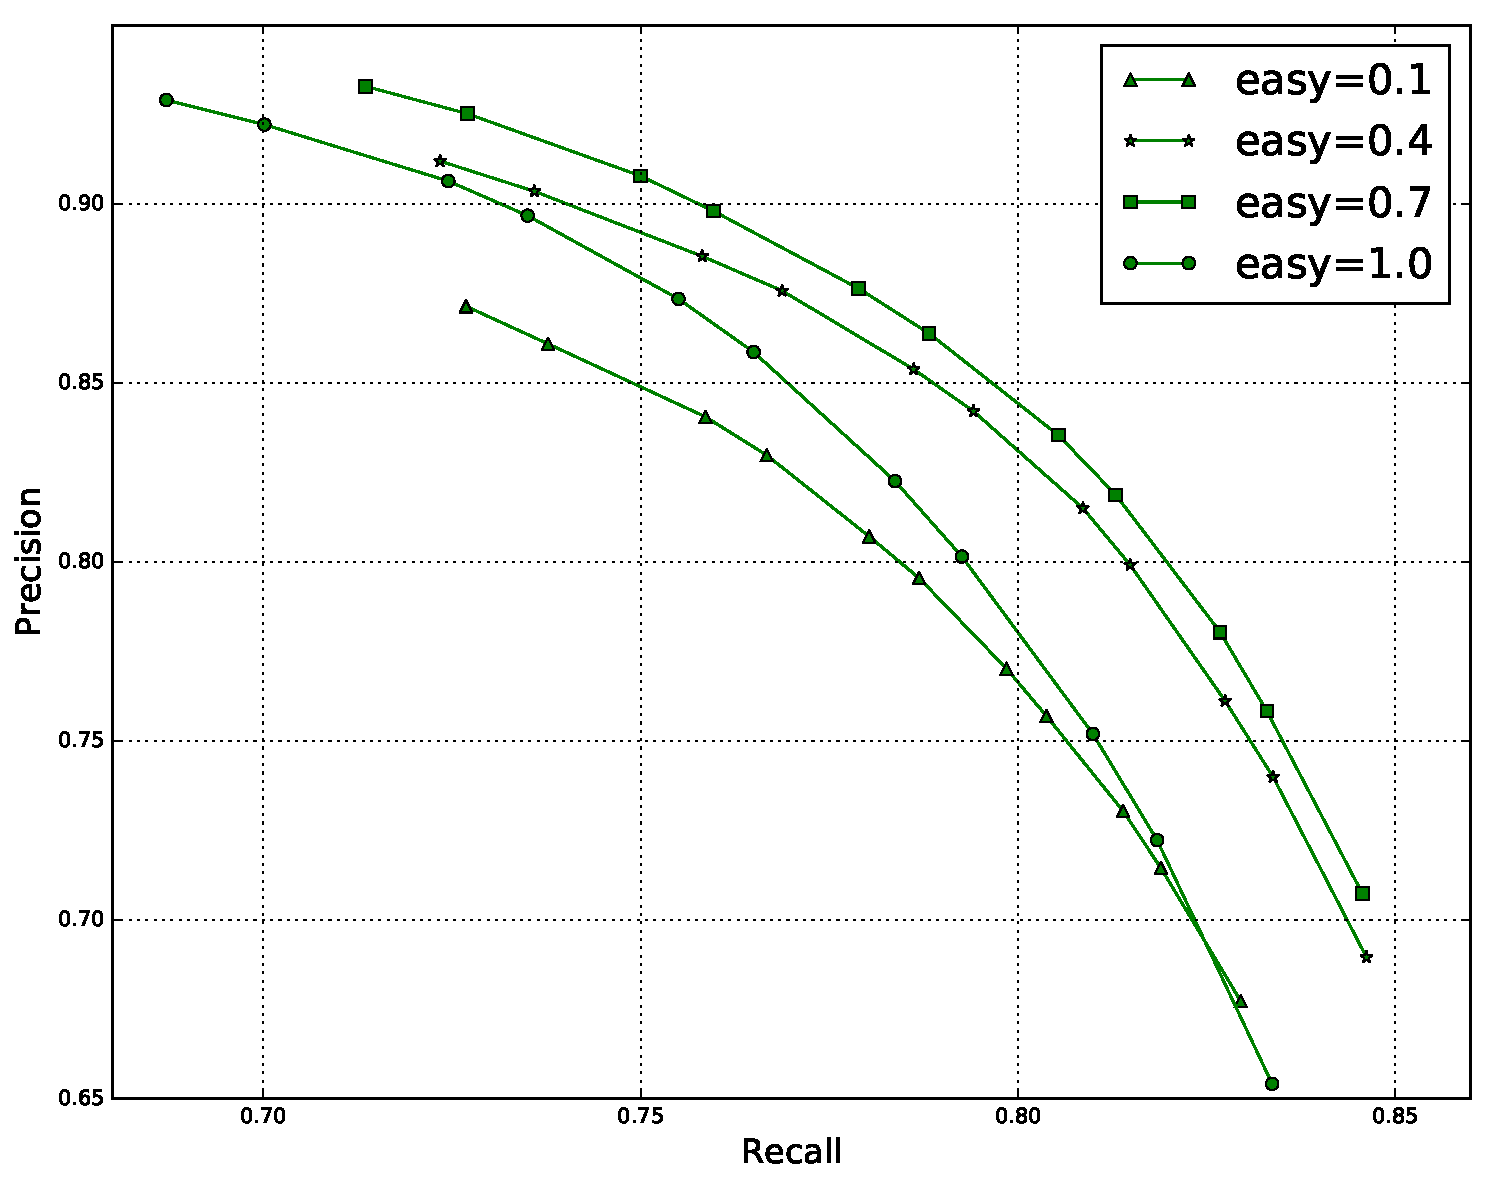
\includegraphics[width=0.5\linewidth]{figures/pr_curve.pdf} \\
  (a)  & (b) \\
\end{tabular}
\caption{(a) Histogram of predicted foreground probabilities using RF. (b) Precision-recall curve for varying thresholded RF mask. Different curves correspond to different annotation budget}
\end{figure}

\section{Bayesian Formulation of segmentation problem}
In this thesis, we make use of prior information to compensate for the lack of sufficient training data and for the uncertainty of RF classifier. To make use of prior, we model our image segmentation problem as a Bayesian inference problem. Let us cosider an observed image, $\mat{I}$ and labeled or segmented ground truth, $\mat{M}$, the joint probabilty can be defined as:
\begin{equation*}
\p(\mat{I}, \mat{M}) = \p(\mat{M}) \p(\mat{I}|\mat{M}) \eqcont
\end{equation*}
and applying Bayes theorem,
\begin{align*}
\p(\mat{M}|\mat{I}) \, & = \frac{\p(\mat{M}) \p(\mat{I}|\mat{M})}{\p(\mat{I})} \\
						& \propto \, {\p(\mat{M}) \p(\mat{I}|\mat{M})}
\end{align*}
The left hand side is the probability of obtaining segmentation mask, $\mat{M}$ given the image $\mat{I}$, is called the posterior probability. $\p(\mat{M})$ is the prior probability of mask, $\mat{M}$. The Maximum a posteriori (MAP) estimate, $\mat{M^*}$ can be calculated as follow:
\begin{equation}
\mat{M^*} = \arg\max_{\mat{M}}{\p(\mat{M}) \p(\mat{I}|\mat{M})} \eqend
\end{equation}

The above problem can as well be stated as an energy minimization problem by
writing Equation 3.1 in terms of energy by taking negative log-likelihood:
\begin{align*}
\funop{E}(\mat{M}) &=\, - \, \log(\p(\mat{I}, \mat{M})) \\
&= -\, \log(\p(\mat{I}|\mat{M})) - \log(\p(\mat{M})) \\
&= \funop{E_d}(\mat{I}, \mat{M}) + \funop{E_r} (\mat{M})
\end{align*}
The total energy, $\funop{E}$, that we want to minimize can be considered as linear combination of data or likelihood term, $\funop{E_d}$, and prior term or regularization, $\funop{E_r}$. This modifies calculating MAP estimate to:
\begin{equation*}
\mat{M^*} = \arg\min_{\mat{M}}{\funop{E_d}(\mat{I}, \mat{M}) + \funop{E_r} (\mat{M})} \eqend
\end{equation*}
To obtain MAP estimate, we need to formulate likelihood term and prior term. We formulate the prior using Total variation(TV). We can find use of different TV priors such as Wulff shapes etc. In our thesis, as the objects we need to segment are smooth and shaped like a circle, we make use of isotropic total variation, $\funop{TV}$. Also, we can try to use isotropic total variation in 2D or 3D as the data we are trying to segment is a 3D stack. For likelihood term, G. Paul et al.\cite{Paul2013} proposed an energy formulation which is not derived from a statistical model but learnt from training set. This gives the advantage of combining example-based and model-based approaches. Similar to Eugster \cite{dominic}, we formulate the likelihood term using a cost function, $\funop{C}$. The likelihood term is formulated as a product of cost function and mask. The cost function assigns a cost depending on predicted foreground probabilities obtained from RF. Let $\p$ be the probability of pixel being foreground (learnt from RF), and $\mat{M}$ be the optimal mask to be estimated, the energy minimization problems becomes:

\begin{align*}
\funop{E}(\mat{M}) &=\, - \, \log(\p(\mat{I}, \mat{M})) = -\, \log(\p(\mat{I}|\mat{M})) - \log(\p(\mat{M})) \\
&= \funop{E_d}(\mat{I}, \mat{M}) + \funop{E_r} (\mat{M})\\
&= \langle\mathcal{C}(\p), \mat{M}\rangle + \lambda\, \funop{TV}(\mat{M}) + \iota_{[0,1]}(\mat{M}) \numberthis \label{eqn}
\end{align*}

where $\mathrm{i}_{[0,1]}(\mat{M})$ is an indicator function to ensure values of $\mat{M}$ remain in [0,1]. In addition to use of cost function as explained in Eugster \cite{dominic}, we enforce a constraint in our energy minimization problem to obtain correct mask values for the pixels annotated by experts as foreground and background. This constraint was not enforced by Eugster \cite{dominic}. We used an indicator function, $\mathrm{i}_{\mathcal{FG}}(\mat{M})$, to ensure pixels in foreground scribbles have value of 1 in mask, and indicator function, $\mathrm{i}_{\mathcal{BG}}(\mat{M})$, to ensure pixels in background scribbles have value of 0 in mask. Using discrete implementaion of TV, the final energy minimization problem becomes:

\begin{align}
\funop{E}(\mat{M}) = \langle\mathcal{C}(\mat{P}), \mat{M}\rangle + \lambda\, \funop{TV}(\mat{M}) + \iota_{[0,1]}(\mat{M}) + \iota_{\mathcal{FG}}(\mat{M})  + \iota_{\mathcal{BG}}(\mat{M}) 
\end{align}
The optimization problem is solved using Alternating Split Bregman method (ASB), as described in Eugster \cite{dominic}. The advantage of using ASB is that it splits the above problem into subproblems. Each subproblem is easy to solve and can be solved independently. Due to this reason, the new constraints for scribbles can be easily coupled with one of the subproblem or can be solved separately. For our formulation, we are able to couple the new constraints with constraint on mask values. The final solution to the problem is obtained by iterating updates. The details of implementation and solution can be obtained from Eugster \cite{dominic}. 


\subsection{Anti-log cost functions}
The cost function has to be defined such that it assigns a positive cost to probabilities less than 0.5 and negative cost to probabilities greater than 0.5. This ensures that the pixels with low probability get a mask value of 0 and reverse for pixels with high probability. We make use of use of \textit{anti-log} cost function explained by Eugster \cite{dominic} and conduct different experiments. The \textit{anti-log} cost function is defined as:

\begin{align*}
\mathcal{C}(\widehat{p}(x_{k})) =
\begin{cases}
  0, & \text{if}\ x_k \in \mathcal{S}  \\
  -\log \frac{\widehat{\p}(x_{k})}{1-\widehat{\p}(x_{k})}, & \text{else} 
\end{cases} \eqcont
\end{align*} 

where $\mathcal{S}$ corresponds to set of annotated pixels and $\widehat{p}(x_{k})$ is the probability learnt from RF at pixel, $x_k$. The plot of \textit{anti-log} cost function can be seen in figure 3.7. We can observe that cost tends to positive infinity for probablity values close to 0 and, to negative infinity for probablity close to 1. The pixels with values exactly equal to 0 and 1 are given cost of zero and added to $\iota_{\mathcal{FG}}(\mat{M})$ and $\iota_{\mathcal{BG}}(\mat{M})$ respectively for implementation purpose.

\begin{figure}[h!] \label{fig:nll}
\centering
 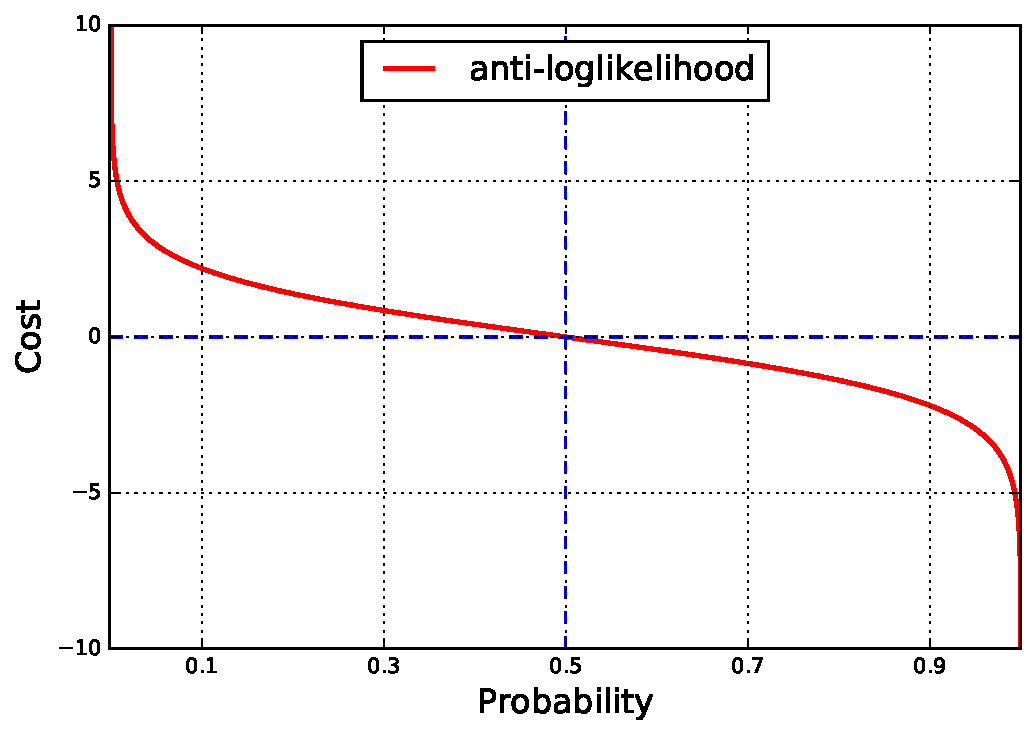
\includegraphics[width=0.75\linewidth]{figures/nll_func.pdf}
\caption{Anti-log cost function}
\end{figure}

To observe the effect of using prior, we repeated the previous experiment of addition of "easy" scribbles and "hard" scribbles in steps. But instead of measuring segmentation accuracy on thresholded RF output mask, we used the predicted RF probabilities to obtain a cost function and obtain the MAP estimate solving equation 3.2. The experiment was conducted for a range of regularization parameter ($\lambda$).


\begin{figure}[h!] \label{fig:rf_vip}
\centering
 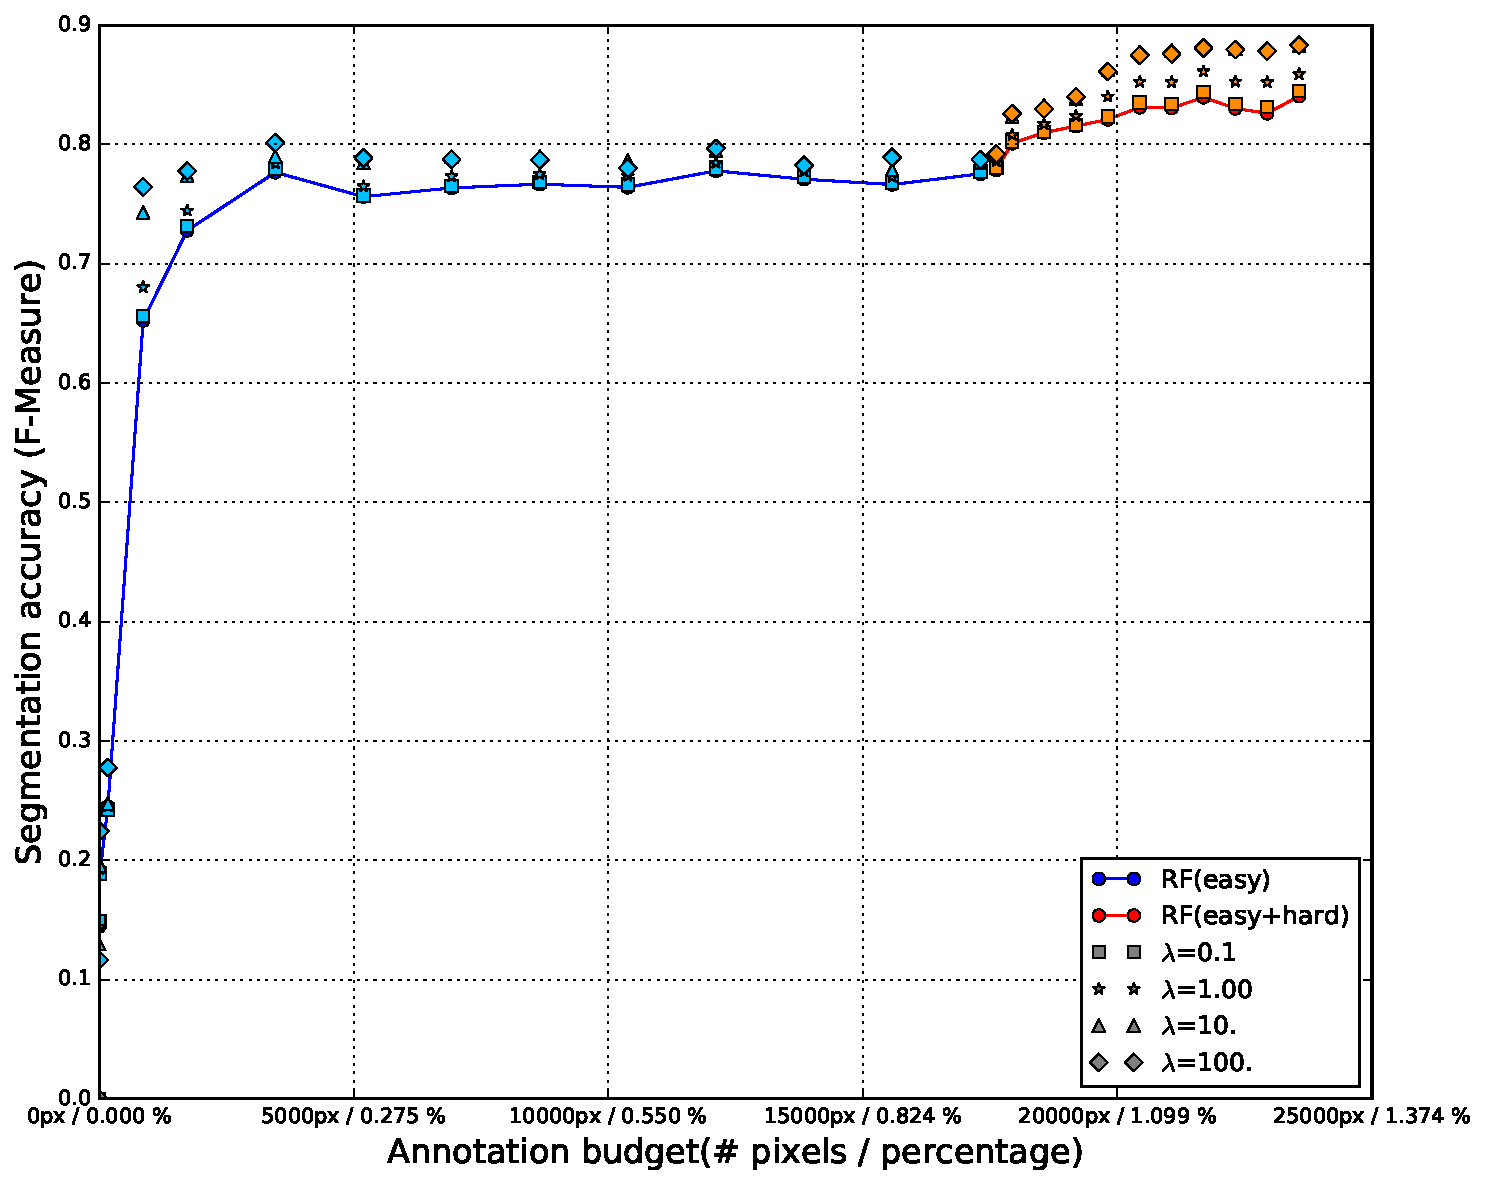
\includegraphics[width=0.75\linewidth]{figures/rf_vip_easy_hard_full.pdf}
\caption{Segmentation score with RF and prior(TV) for different annotation budget}
\end{figure}

\begin{figure}[h!] \label{fig:rf_vip}
\centering
 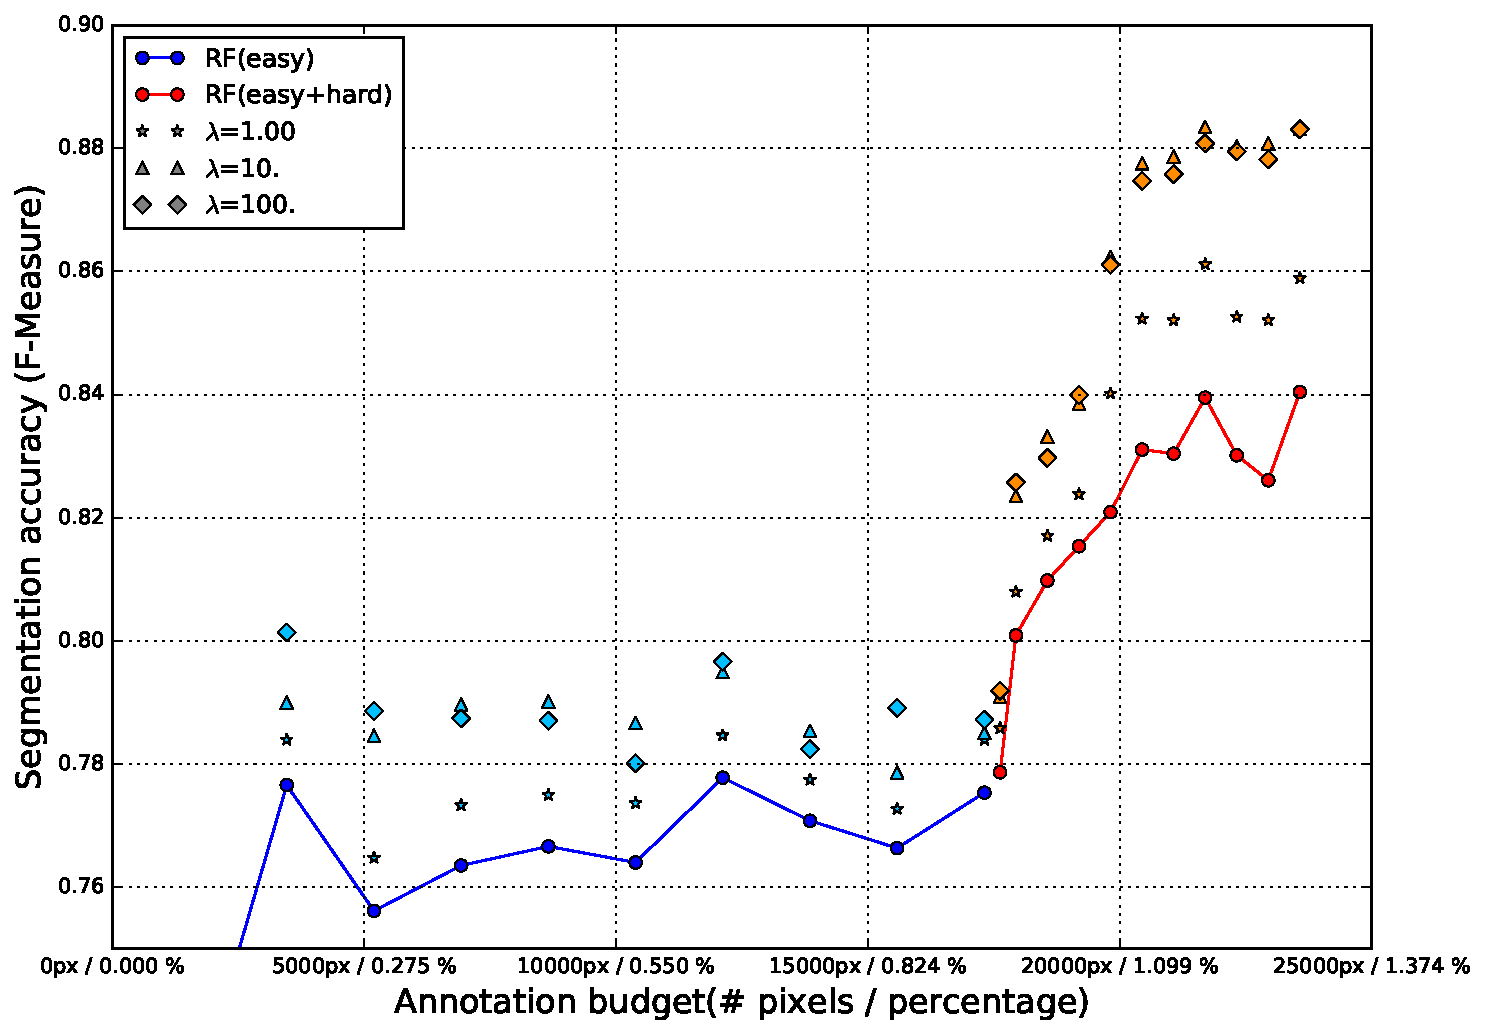
\includegraphics[width=0.75\linewidth]{figures/rf_vip_easy_then_hard.pdf}
\caption{Segmentation score with RF and prior(TV) for different annotation budget (removing very annotation budgets)}
\end{figure}

The results for RF with variational image processing (VIP) can be seen in figure 3.8. We can observe an improvement due to the use of the variational method. Even for very small annotation budget as 0.1\%, we observe an improvement with the use of VIP. Figure 3.9 shows the improvement more clearly for different values of $\lambda$. We can observe that the value of $\lambda$ giving maximum improvement is different for different annotation budgets. 

The use of prior information boosts up the performance but we get different boost for different value of $\lambda$. The regularisation parameter decides the weight of TV cost. One expects smooth boundaries in segmentation mask for high values, but this also effect mask for small objects. We can observe this in figure 3.9. The upper row shows that for larger vesicles, the boundary gets smooth for higher values of $\lambda$, while the bottom row shows that tiny vesicles in image tend to diminish for high values of $\lambda$. This shows that the ideal case will be to choose different $\lambda$ for different part of images or to combine results for different $\lambda$. 

\begin{figure}[h!] \label{fig:effect}
 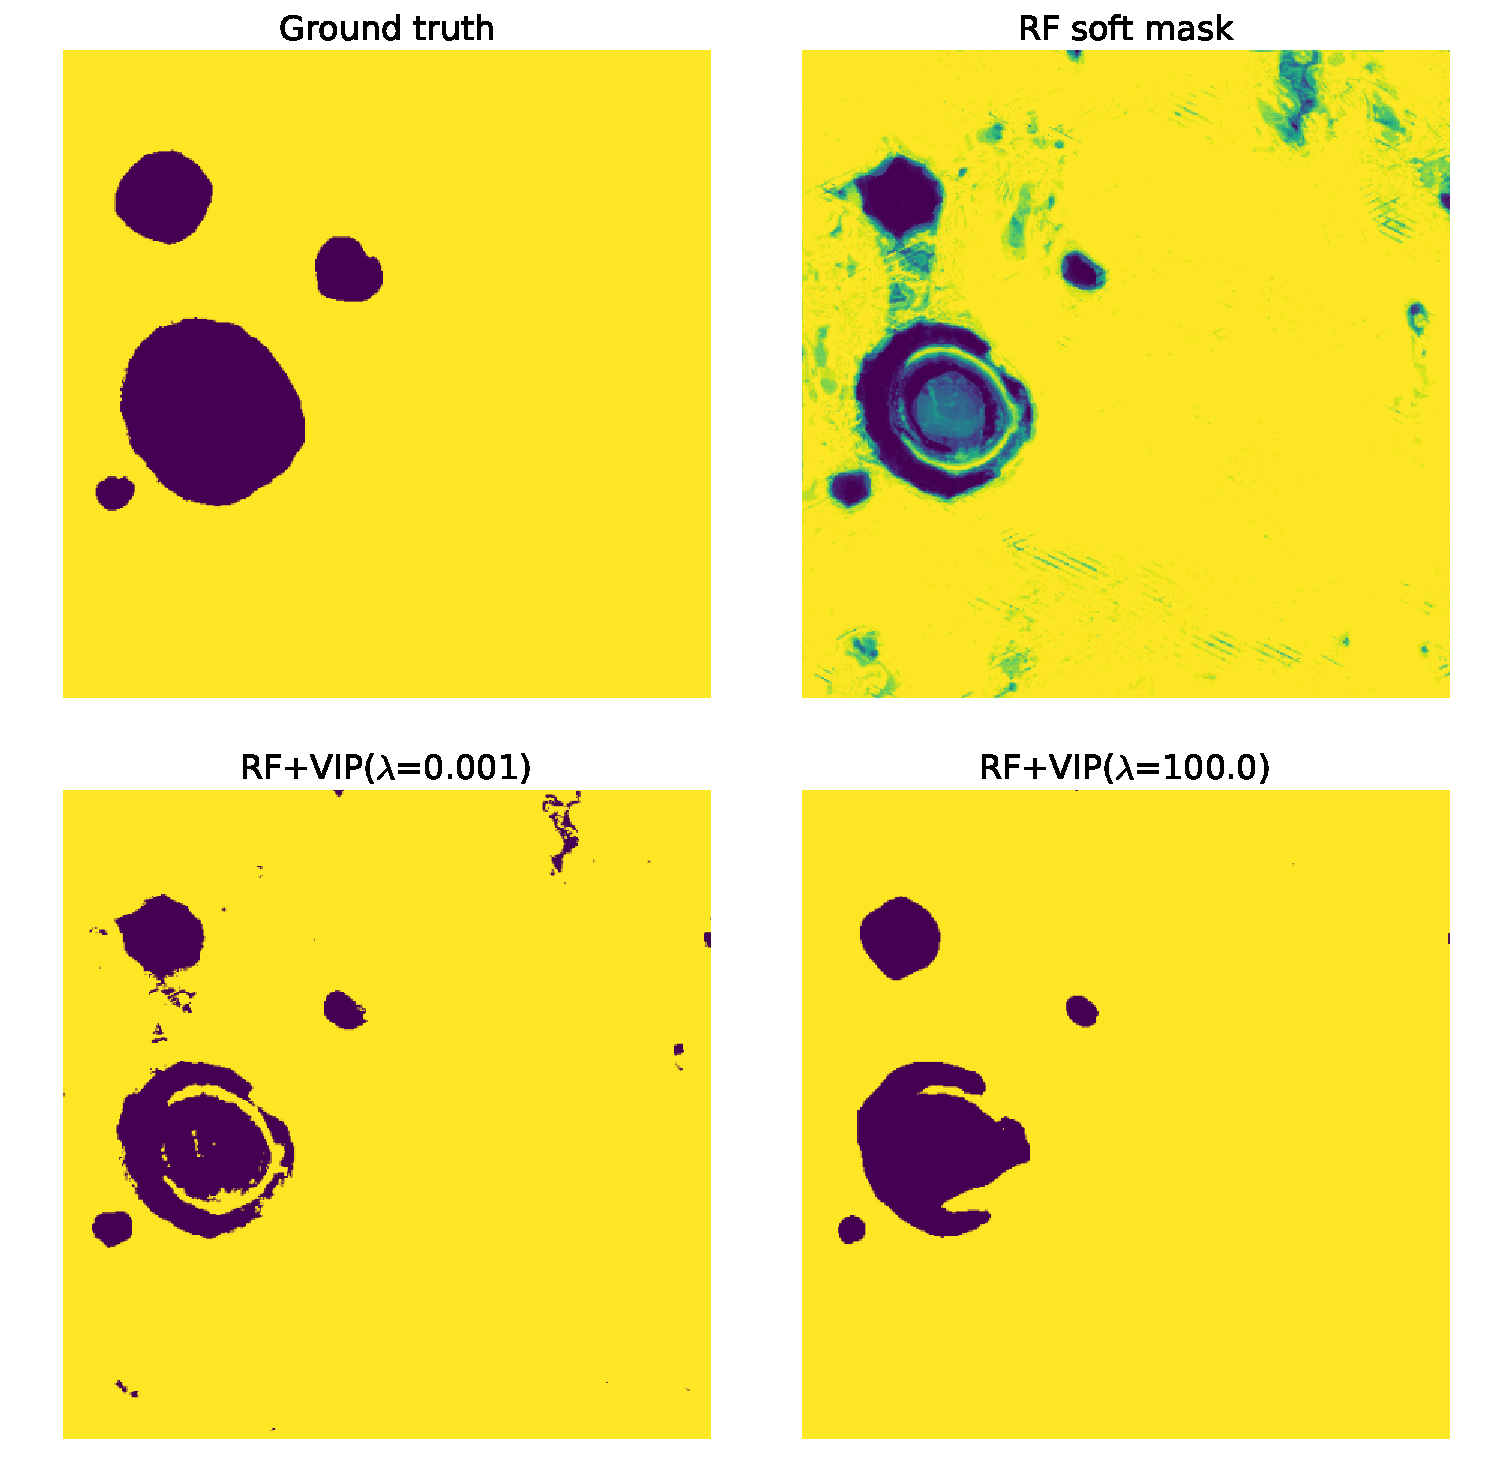
\includegraphics[width=1.0\linewidth]{figures/lamda_effect.pdf}
\caption{Segmentation mask for differnt $\lambda$ for 2 crops of image}
\end{figure}


\subsection{Comparing different cost functions}
In literature, people have used different cost functions to formulate likelihood term.
Santner \cite{santner:2009} makes use a linear cost function to formulate likelihood. The exact functional form in terms of probability is not given in \cite{santner:2009}. Therefore, for our purpose of comparing results, we choose the \textit{linear} cost function as given below:
\begin{align*}
\funop{C_l}(\mat{P}) = -4\,(\mat{p}-0.5) \eqend
\end{align*}
The above function is chosen to show a behaviour similar to \textit{anti-log} cost function at probablity of 0.5. The slope of 4 is selected to match the slope of \textit{anti-log} cost function at 0.5. In addition to the cost function, Santner \cite{santner:2009} mentioned use of hard constraint for pixels in foreground or background scribbles i.e. using cost of $-\infty$ for foreground scribbles and $\infty$ for background scribbles. They didn't show a way to enforce this constraint with \textit{linear} cost function. We enforce this constraint with use of indicator functions, $\iota_{\mathcal{FG}}(\mat{M})$ and $\iota_{\mathcal{BG}}(\mat{M})$. \par
To compare results of these different cost functions, we designed a similar experiment to observe effect of annotation budget on their usage. Instead of choosing pixels from scribbles, we select the annotated pixels randomly from fully annotated ground truth segmentation mask. We increased the annotation budget from using few pixels to using all pixels for training RF. We generate results to compare 3 cost functions: \textit{anti-log}, \textit{linear} and \textit{linear} (with constraints). The results for these different functions can be observed in figure 3.11, 3.12 and 3.13. The blue dotted line in all these figures shows the accuracy obtained for thresholded RF output mask.

\begin{figure}[h!] \label{fig:nll}
\centering
 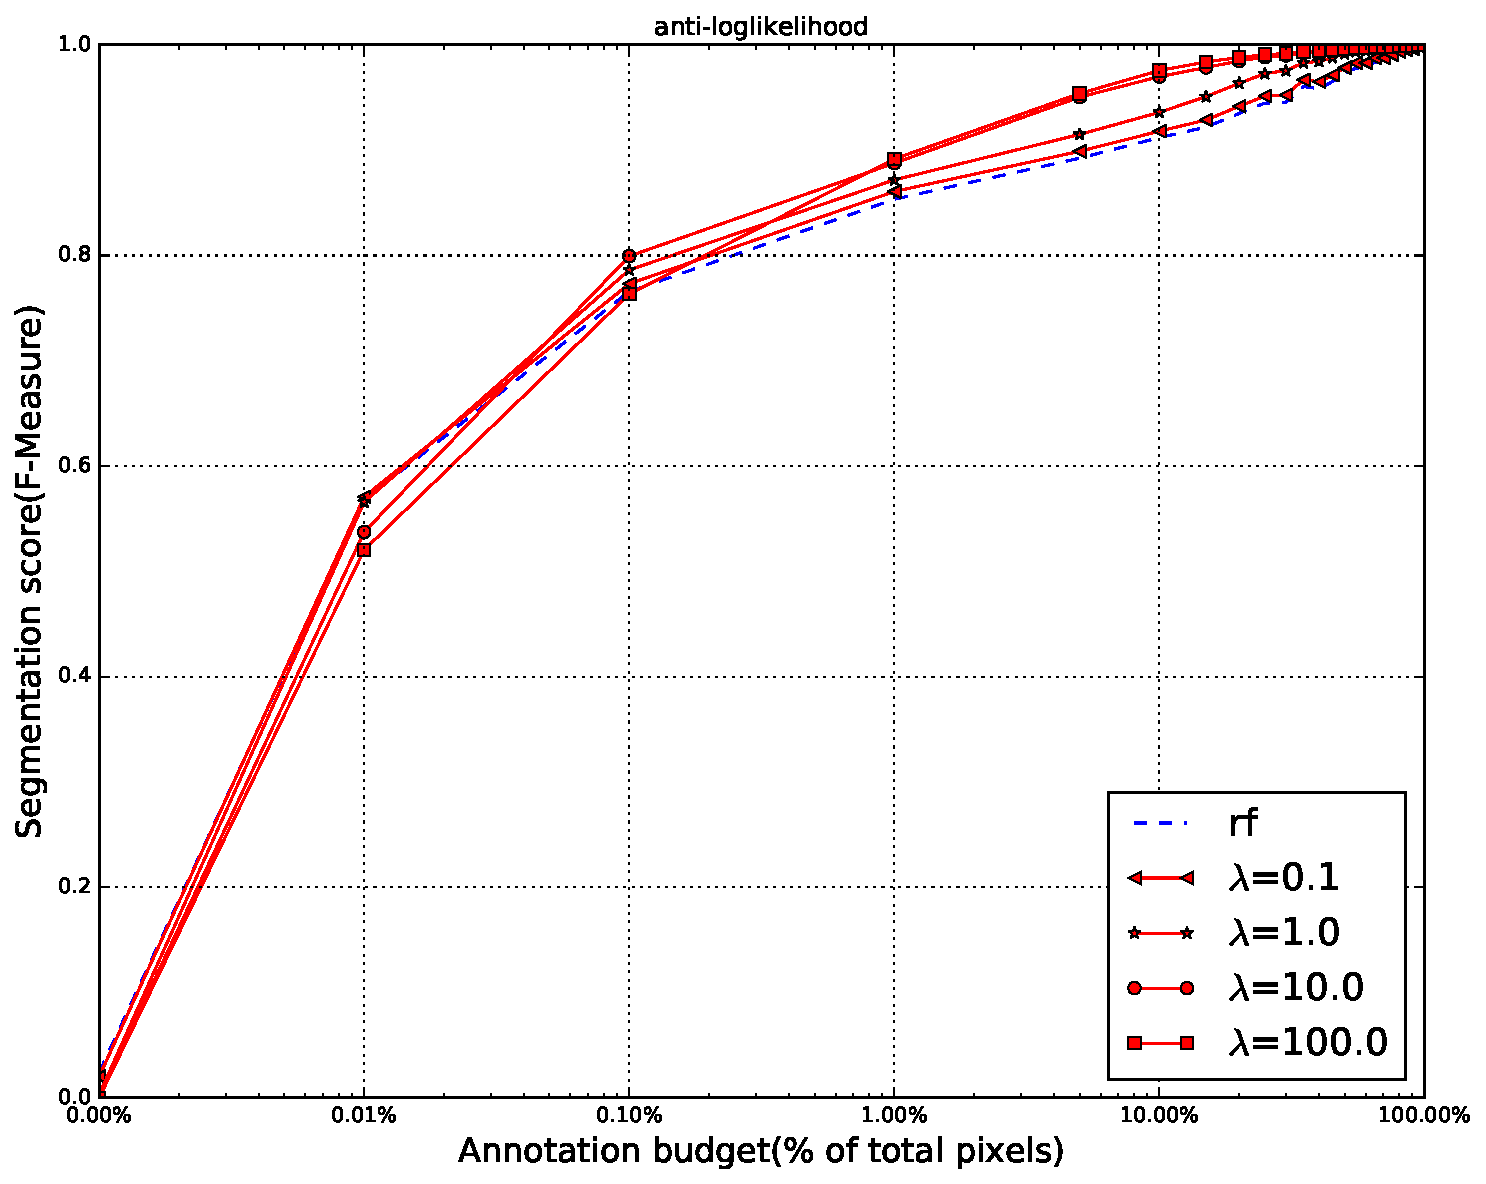
\includegraphics[width=0.75\linewidth]{figures/anti_nll.pdf}
\caption{Segmentation accuracy vs annotation budget for \textit{anti-log} cost function.}
\end{figure}

\begin{figure}[h!] \label{fig:rf_vip2}
\centering
 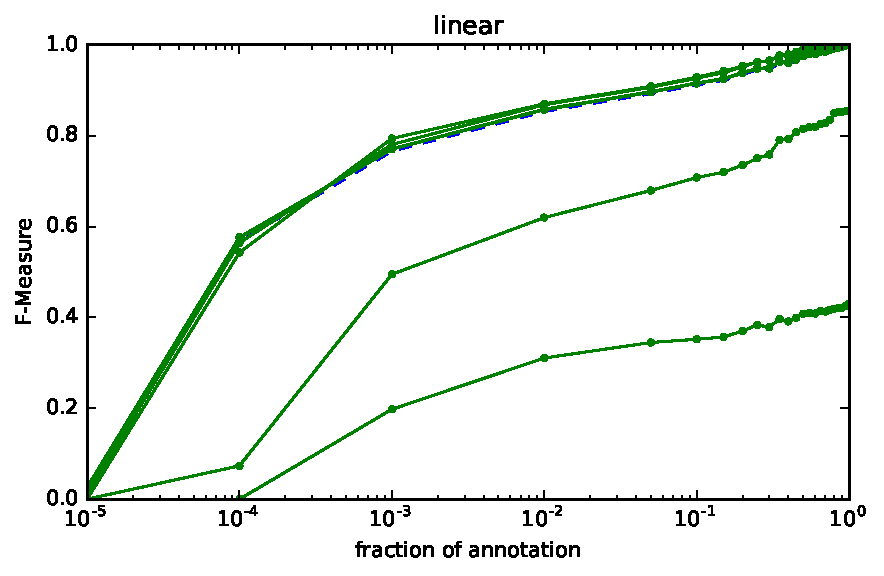
\includegraphics[width=0.75\linewidth]{figures/linear.pdf} 
\caption{Segmentation accuracy vs annotation budget for \textit{linear} cost function.}
\end{figure}

\begin{figure}[h!] \label{fig:rf_vip3}
\centering
 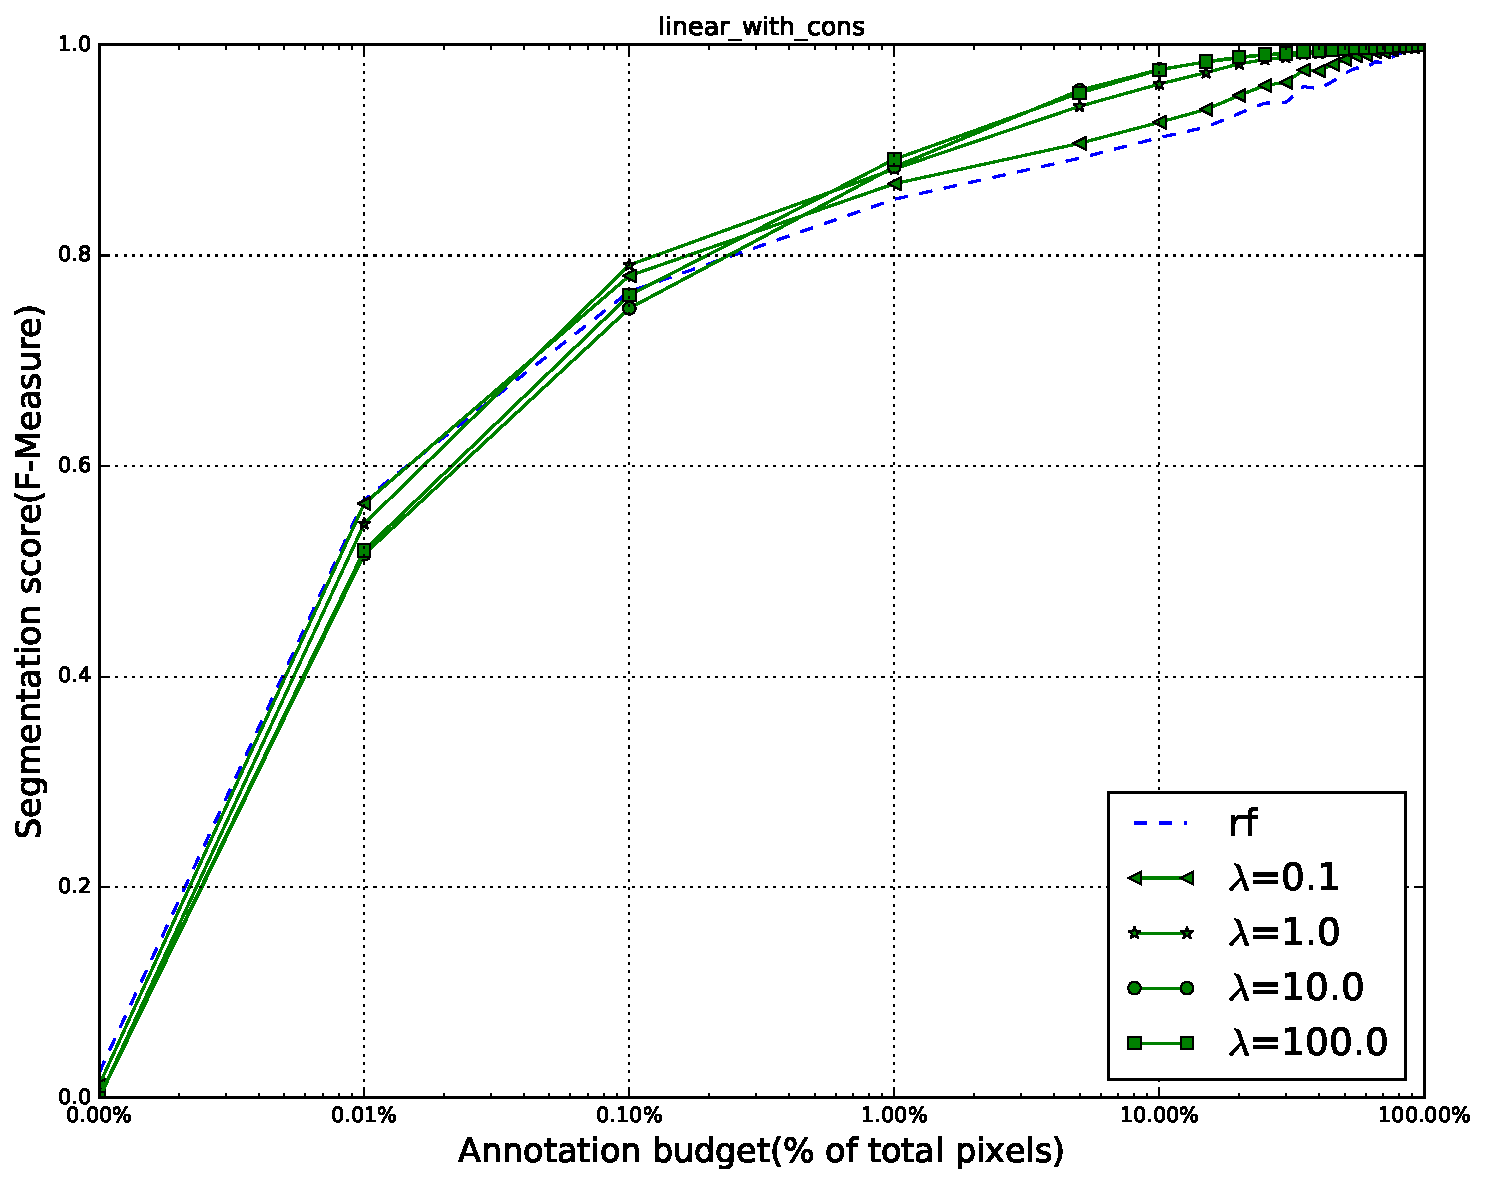
\includegraphics[width=0.75\linewidth]{figures/linear_with_cons.pdf}
\caption{Segmentation accuracy vs annotation budget for \textit{linear} cost function with constraints.}
\end{figure}


Figure 3.11 shows that for all values of $\lambda$, the \textit{anti-log} cost function does not decrease the segmentation accuracy. Only for very low annotation budget (< 0.1\%), the accuracy decreases by a small amount. Else, the use of \textit{anti-log} cost function ensures that the use of VIP does not decrease the accuracy and thus, always improving the output mask obtained from RF. Especially for the higher annotation budgets (> 50\%), the use of constraints does not allow VIP to change mask value for annotated pixels. This shows the robustness of cost function and allows the user to choose values of $\lambda$ freely in a reasonable range. From figure 3.12, we can observe that \textit{linear} cost function does not work well with large values of $\lambda$ and also significanty deteriorates the mask obtained from RF. Even for $\lambda$ equal to 10, the accuracy drop significantly in comparison to accuracy obtained from thresholded RF mask. This shows that while using \textit{linear} cost function, the value of $\lambda$ is to be chosen carefuly. Contrary to results for \textit{linear} cost function, the results for the \textit{linear} cost function with constraints in figure 3.13 is almost similar to the results for \textit{anti-log} cost function. The use of constraints makes it robust and avoids corruption of the mask obtained from RF. In figure 3.14, we foucus on higher values of annotation budgets. It can be seen that the segmentation accuracy for all cost functions converge to 1 with the increment of annotation budget to 100\% i.e. using all pixels in the image for training. The difference can be seen in convergence for the 3 different cost functions. These cost functions shows different amount of improvement for same annotation budget. The effect of the same value of $\lambda$ is also different for these cost functions. It can be seen that \textit{anti-log} and \textit{linear} (with constraints) show maximum and almost same improvement for $\lambda$equal to 100.



\begin{figure}[h!] \label{fig:rf_vip_diff}
% \begin{tabular}{ccc}
 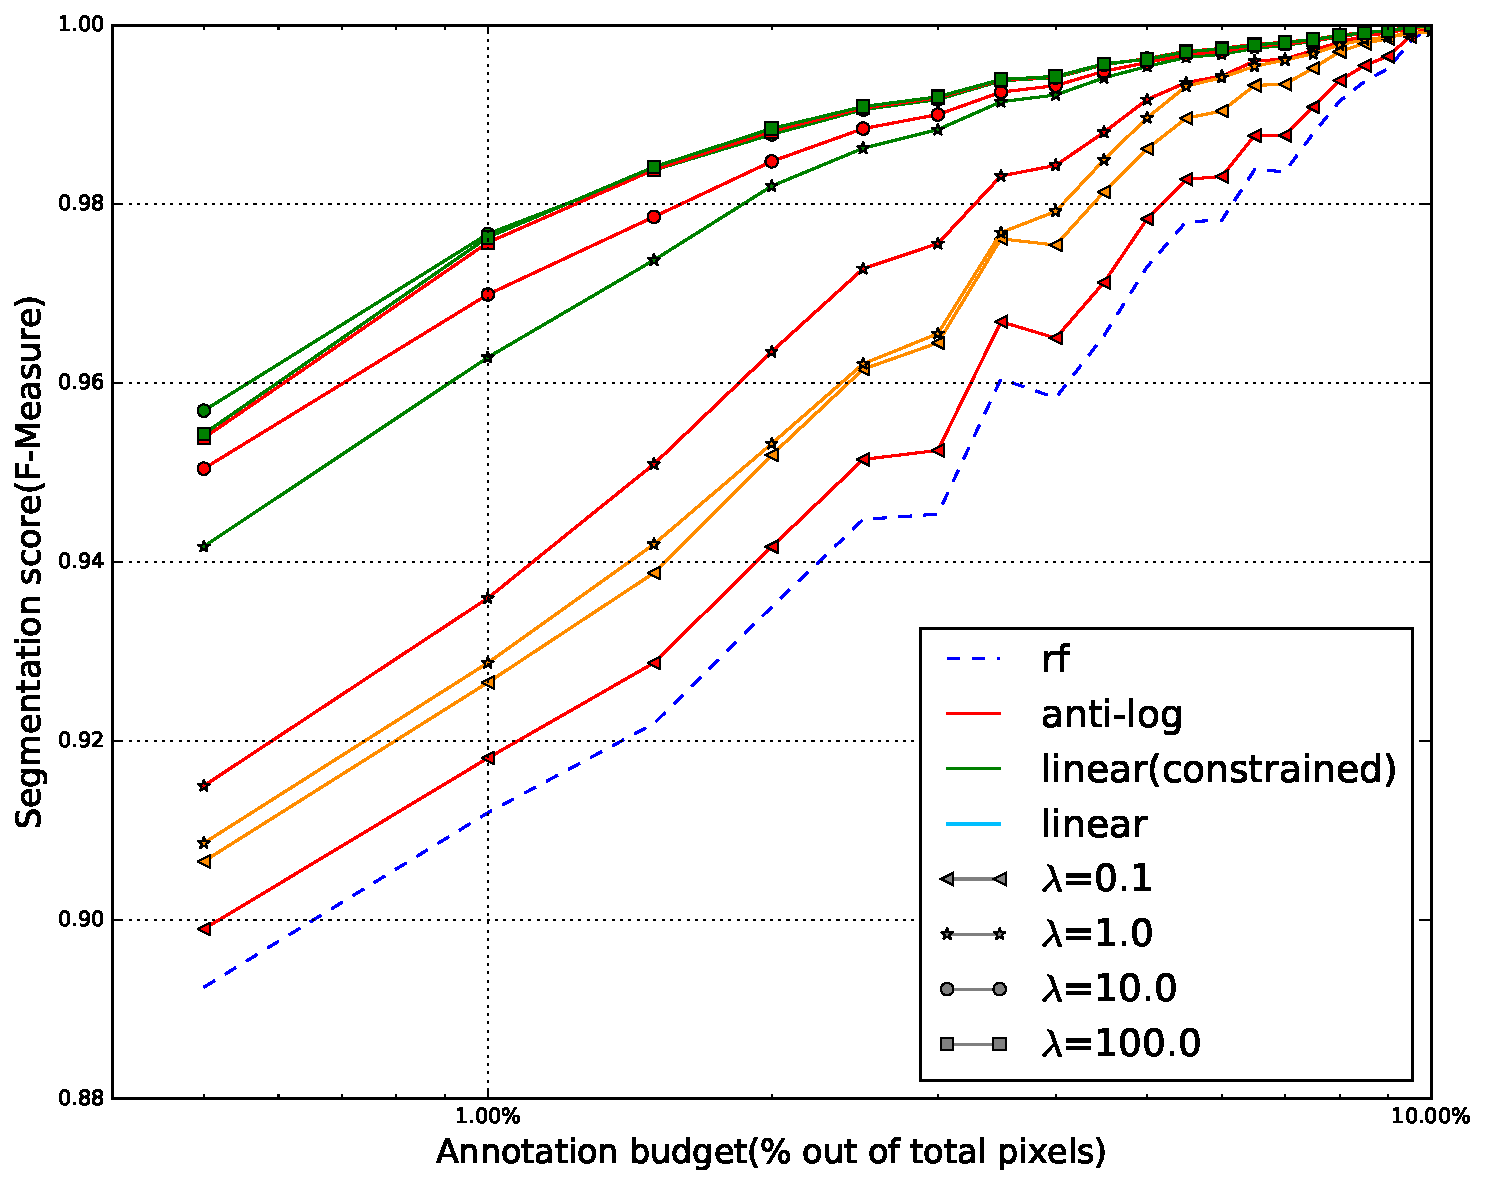
\includegraphics[width=0.75\linewidth]{figures/vip_diff.pdf}
% \end{tabular}
\caption{Comparison of different cost functions for higher annotation budgets.}
\end{figure}



% \subsection{2D vs 3D Total Variation}
% We observed the boost due to use to isotropic TV in 2D. Since the slices form a 3D stack, it is usual to try 3D isotropic TV. We can observe the boost in figure 3.10

\section{Semi-interactive segmentation}
We realized the need for iterative semi-interactive segmentation in section 3.1.2. With 1 iteration of interactive segmentation, we were able to improve f-measure results. Now, we combine semi-interactive annotation with the use of variational segmentation. We take segmentation mask obtained from variational segmentation and add scribbles to image where the RF and VIP together are unable to segment correctly. Then, we retrain Random forest and generate new mask using variational segmentation. The image, mask, and scribbles are shown in figure 3.10. We can observe the improvement in the mask with an addition of only 5000 pixels (less 0.2\% of pixels in the image).
\begin{figure}[h!] \label{fig:semi-vip}
 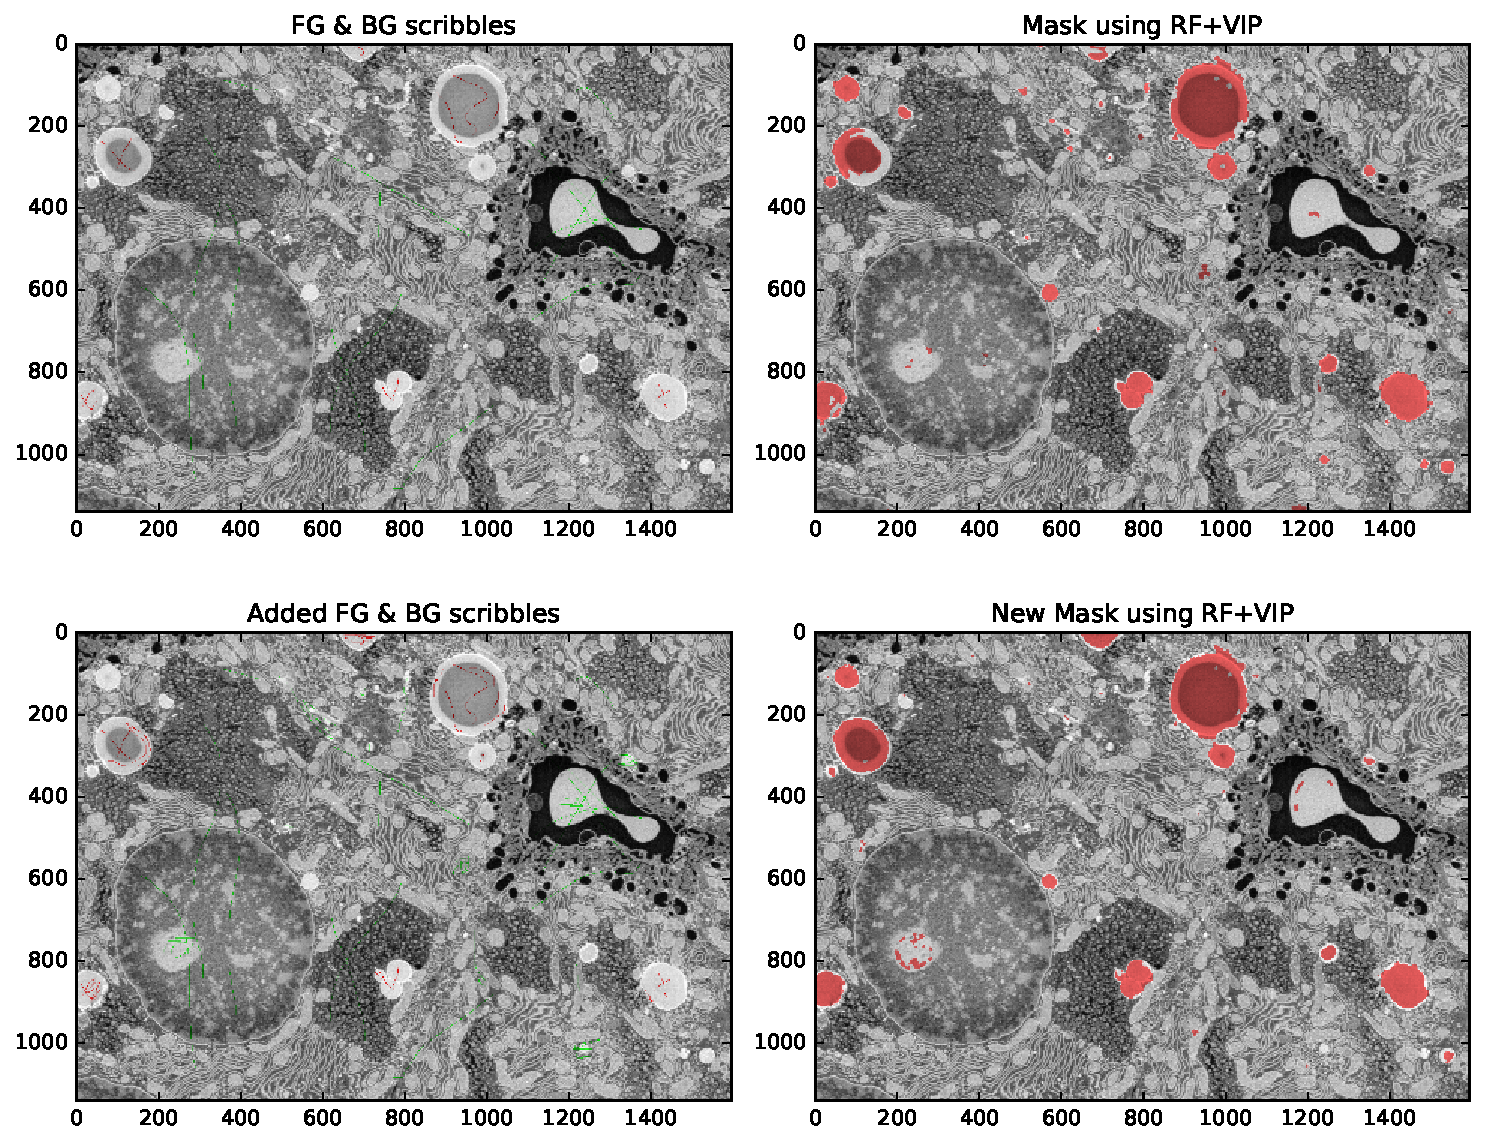
\includegraphics[width=1.0\linewidth]{figures/semi_inter_vip.pdf}
\caption{Semi-interactive segmentation with one iteration (RF+VIP)}
\end{figure}
